\chapter{Ternary Cahn--Hilliard and the phase diagram}
\label{ch:p4}

\begin{keybox}
\textbf{Key idea.} A real cast blend has (at least) three components ---
two solutes and a solvent. With two independent conserved compositions
the free energy is a \emph{surface over the Gibbs triangle}, and demixing
follows \emph{tie-lines} on that triangle. Reading morphology on the
phase diagram, not on a single axis, is the multi-component way of
thinking.
\end{keybox}

\section{The model}

Let $\phi_1,\phi_2$ be the volume fractions of the two solutes; the
solvent is eliminated by $\phi_s = 1-\phi_1-\phi_2$. Each solute carries
a conserved $(\phi_i,\mu_i)$ Cahn--Hilliard pair; the Flory--Huggins
exchange chemical potentials are
%
\begin{equation}
  \mu_i^{\text{bulk}} = \ln\!\frac{\phi_i}{\phi_s}
   + \chi_{12}\,\phi_j + \chi_{is}(\phi_s-\phi_i) - \chi_{js}\,\phi_j,
   \qquad j\neq i,
\end{equation}
%
and the coupled conserved dynamics is
%
\begin{equation}
  \dd{\phi_i}{t} = \grad\!\cdot\!\Big(\textstyle\sum_j M_{ij}\grad\mu_j\Big),
  \qquad \mu_i = \mu_i^{\text{bulk}} - \kappa_i\grad^2\phi_i ,
\end{equation}
%
with $M$ a symmetric positive-definite Onsager mobility matrix (its
off-diagonal couples the two solute fluxes). This is Chapter~\ref{ch:p1}
promoted to two composition fields.

\begin{keybox}
\textbf{Coefficients.} Three interaction parameters:
$\chi_{12}=\PfourChiab$ (solute--solute; large $\Rightarrow$ the two
solutes demix), $\chi_{1s}=\PfourChias$ and $\chi_{2s}=\PfourChibs$
(solute--solvent). The mobility matrix sets the time scale and the
relative solute speeds; $\kappa_i$ set interface widths. Real blends map
these to the $\chi$'s in \file{materials/materials.yaml} (e.g.\ the
P3HT:PCBM and PDPP5T:PCBM systems).
\end{keybox}

\section{The Gibbs triangle}

Each node has a composition $(\phi_1,\phi_2,\phi_s)$ summing to one --- a
point in the 2-simplex, drawn as a point in an equilateral triangle
(barycentric coordinates; solvent, $\phi_1$, $\phi_2$ at the three
vertices). The bulk \emph{average} is conserved and never moves; the
\emph{cloud} of local compositions starts as a tight blob at the initial
blend and, as the system demixes, opens up along a tie-line toward the
two coexisting phases. Watching that cloud open \emph{is} watching
ternary phase separation.

\section{Run it}

\begin{runbox}
\textbf{Run it.}
\begin{lstlisting}
cd physics/04_ternary_ch_phase_diagram
python run.py            # ternary spinodal quench
\end{lstlisting}
It marches a ternary quench from a homogeneous blend
$(\phi_1,\phi_2)=(\PfourPhione,\PfourPhitwo)$ and reports how the
composition cloud spreads and where the two coexisting phases land.
Compare with \file{EXPECTED.md} and the Gibbs-triangle figure.
\end{runbox}

\paragraph{What you should see.} The composition spread grows from
$\PfourSpreadStart$ (a tight initial blob) to $\PfourSpreadEnd$ as the
blend separates into two phases at $\PfourPhaseA$ and $\PfourPhaseB$ (in
$(\phi_1,\phi_2)$). The mean composition stays pinned to solver
tolerance ($|\Delta\phi|\le\PfourDrift$): conservation fixes the
\emph{centroid} of the cloud while it opens along the tie-line.

% --- generated by gen_figures.py ---
\begin{figure}[h]\centering
  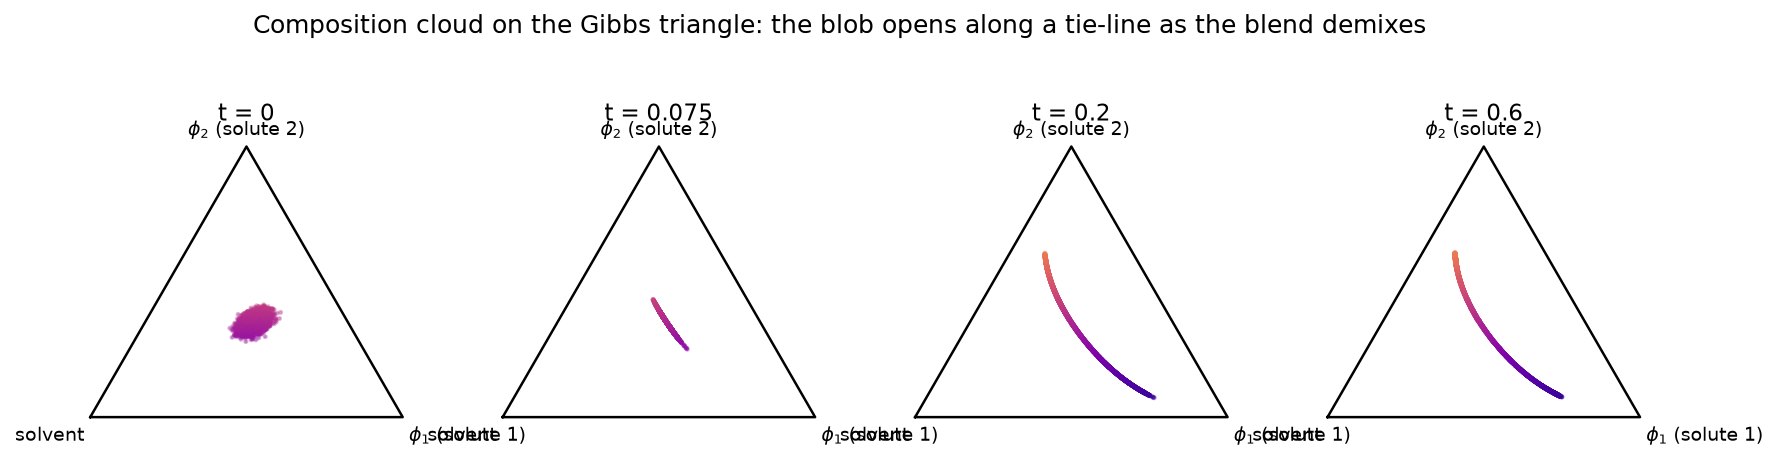
\includegraphics[width=\linewidth]{figures/p4_gibbs.png}
  \caption{Composition trajectory on the Gibbs triangle: the local-
    composition cloud (one point per mesh node) opens from the initial
    blend along a tie-line toward the two coexisting phases. The mean
    (centroid) is conserved.}
  \label{fig:p4gibbs}
\end{figure}

\begin{figure}[h]\centering
  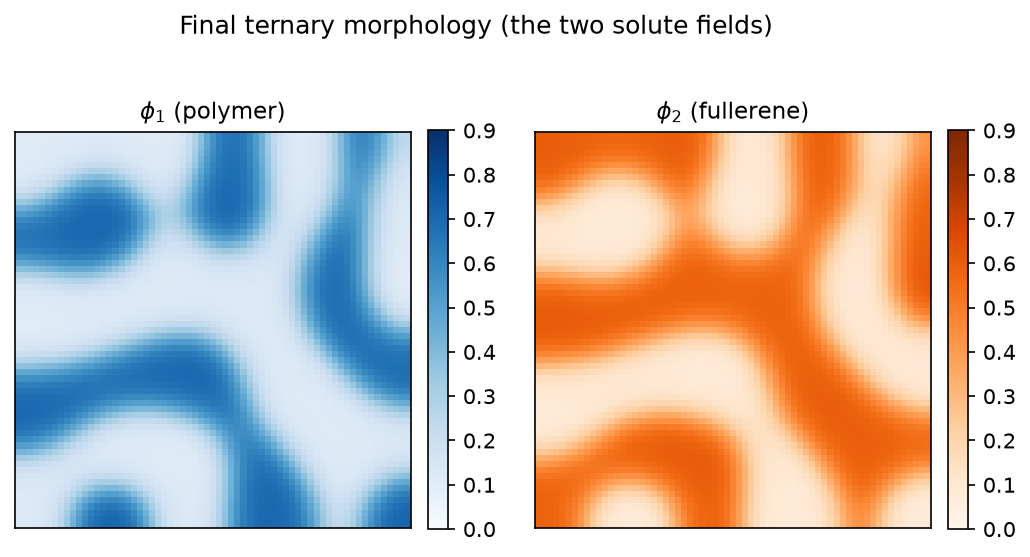
\includegraphics[width=0.85\linewidth]{figures/p4_fields.png}
  \caption{The two solute fields of the final ternary morphology.}
  \label{fig:p4fields}
\end{figure}

\begin{keybox}
\textbf{Measured self-check.}
\begin{center}\small
\begin{tabular}{lc}
\toprule
composition spread (std $\phi_1$): start $\to$ end & $\PfourSpreadStart \to \PfourSpreadEnd$ \\
coexisting phase A $(\phi_1,\phi_2)$ & \PfourPhaseA \\
coexisting phase B $(\phi_1,\phi_2)$ & \PfourPhaseB \\
mean drift $|\Delta\phi|$ & \PfourDrift \\
\bottomrule
\end{tabular}
\end{center}
\end{keybox}

\section{Code walk-through}

\paragraph{1. The ternary stepper.} \code{TernaryCHStepper(dm, chi=(...),
M=(...), kappa=(...))} builds the four-field $(\phi_1,\mu_1,\phi_2,\mu_2)$
system; \code{set\_initial(f1, f2)} seeds the two compositions.

\paragraph{2. Barycentric projection.} \code{bary\_to\_xy(phi1, phi2)}
maps a composition to triangle coordinates; scattering every node gives
the cloud of Fig.~\ref{fig:p4gibbs}.

\paragraph{3. Tie-line readout.} Splitting the final field at the median
$\phi_1$ and averaging each half estimates the two coexisting phase
compositions (the tie-line endpoints).

\section{Explore on your own}

\question{Increase $\chi_{12}$ (make the two solutes more immiscible).
How do the tie-line endpoints move on the triangle, and does the cloud
open further? Where is the spinodal boundary for this blend?}

\question{Change the solvent selectivity: make $\chi_{1s}\neq\chi_{2s}$.
Which solute segregates preferentially, and how does the tie-line
\emph{tilt} on the triangle?}

\question{Shift the initial blend off the symmetric point (e.g.\ solute-
rich). Does the morphology change from bicontinuous to droplet, and does
the cloud still open along the same tie-line?}

\question{The off-diagonal mobility $M_{12}$ couples the two fluxes. Set
it to zero and compare the coarsening: does the morphology or only the
rate change?}

\question{Map a real system from \file{materials.yaml} (say P3HT:PCBM)
onto $(\chi_{12},\chi_{1s},\chi_{2s})$ and predict, from the triangle,
which two phases should coexist. Then run it and check.}

% ====================================================================
